\documentclass{article}
\usepackage{graphicx}

\begin{document}

\title{Simples artigo com lista de figuras}

\author{Joenio Costa}

\maketitle

\section{Lorem ipsum dolor sit amet}

Lorem ipsum dolor sit amet, consectetur adipiscing elit. Donec a diam aenean
ut gravida lorem.

\begin{figure}[h]
\center

\includegraphics[scale=0.3]{gitlab.png}
\caption{Logotipo do Gitlab}
\end{figure}

\begin{table}
  \begin{tabular}{ l c r }
    1 & 2 & 3 \\
    4 & 5 & 6 \\
    7 & 8 & 9 \\
  \end{tabular}
  \caption{Tabela simples}
\end{table}

Ut turpis felis, pulvinar a semper sed, adipiscing id dolor.

\begin{figure}[h]
\center
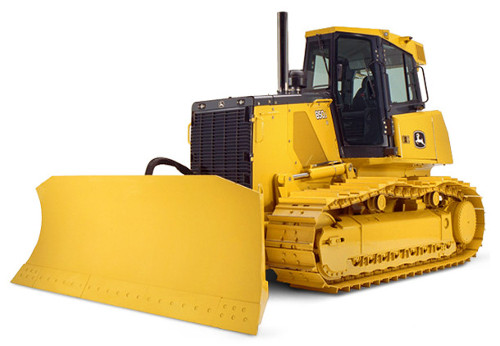
\includegraphics[scale=0.3]{trator.jpg}
\caption{Foto de trator}
\end{figure}

Pellentesque auctor nisi id magna consequat sagittis. Curabitur dapibus enim
sit amet elit pharetra tincidunt feugiat nisl imperdiet.

\begin{figure}[h]
\center

\includegraphics[scale=1.0]{heckert_gnu_small.png}
\caption{Logo do projeto GNU}
\end{figure}

Ut convallis libero in urna ultrices accumsan. Donec sed odio eros.

\begin{table}
  \begin{tabular}{|l|c|r|}
    \hline
    1 & 2 & 3 \\ \hline
    4 & 5 & 6 \\ \hline
    7 & 8 & 9 \\ \hline
  \end{tabular}
  \caption{Tabela com linhas}
\end{table}

\listoffigures
\listoftables
\end{document}
